


\begin{frame}
  \frametitle{In close collaboration with ... }

 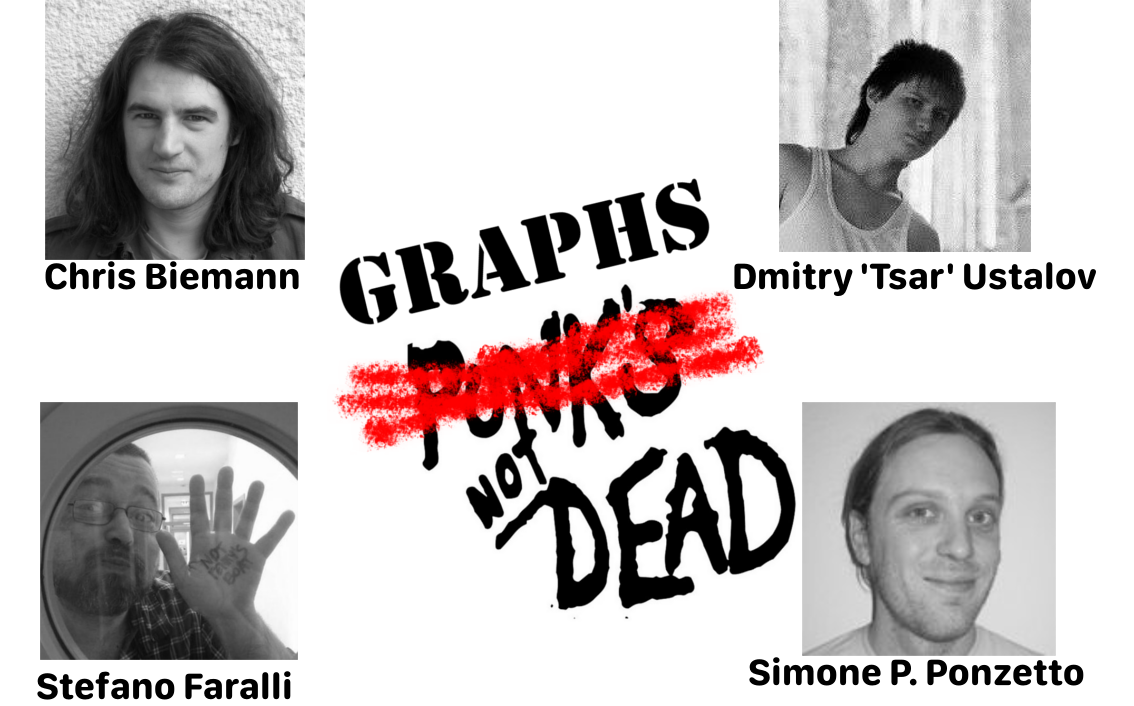
\includegraphics[width=.95\textwidth]{figures/collaborators}	
\end{frame}



\begin{frame}
  \frametitle{In collaboration with ... }
  { \large \bf
  \begin{itemize}
  	\item Andrei Kutuzov
  	\item Eugen Ruppert
  	\item Fide Marten
  	\item Nikolay Arefyev
  	\item Steffen Remus
  	\item Martin Riedl
  	\item Hubert Naets
   	\item Maria Pelevina
	\item Anastasiya Lopukhina
	\item Konstantin Lopukhin
  
  \end{itemize}	
  }
\end{frame}


\section{Motivation}





\begin{frame}{Levels of Linguistic Analysis}
	\vspace{-15pt}
	
  \begin{center}
  	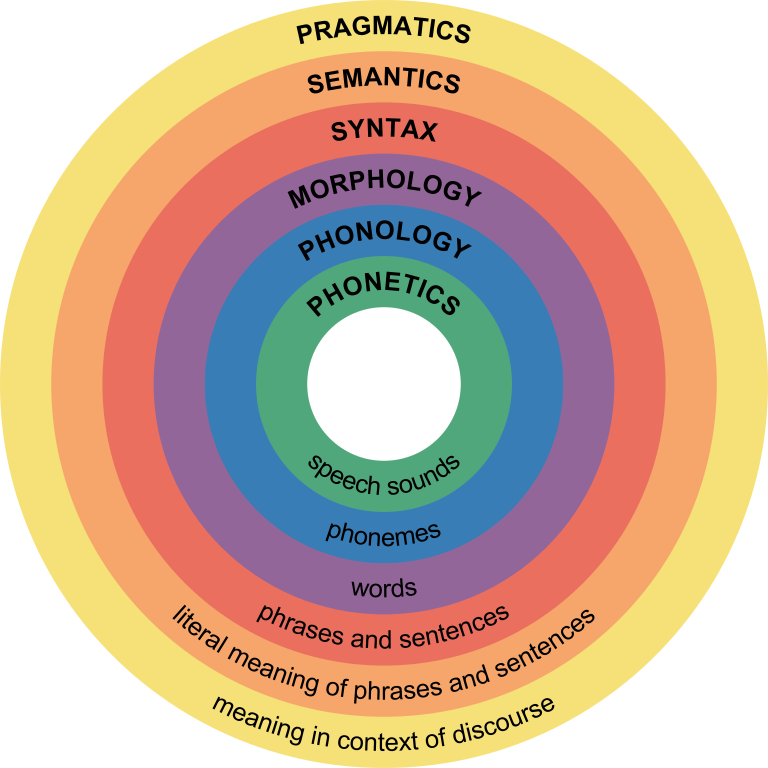
\includegraphics[width=0.5\textwidth]{figures/levels}
  \end{center}
   
{  \tiny
  Image source: \url{https://commons.wikimedia.org/wiki/File:Major_levels_of_linguistic_structure.svg}
 } 

\end{frame}



\begin{frame}{Levels of Linguistic Analysis}
	\vspace{-15pt}
	
  \begin{center}
  	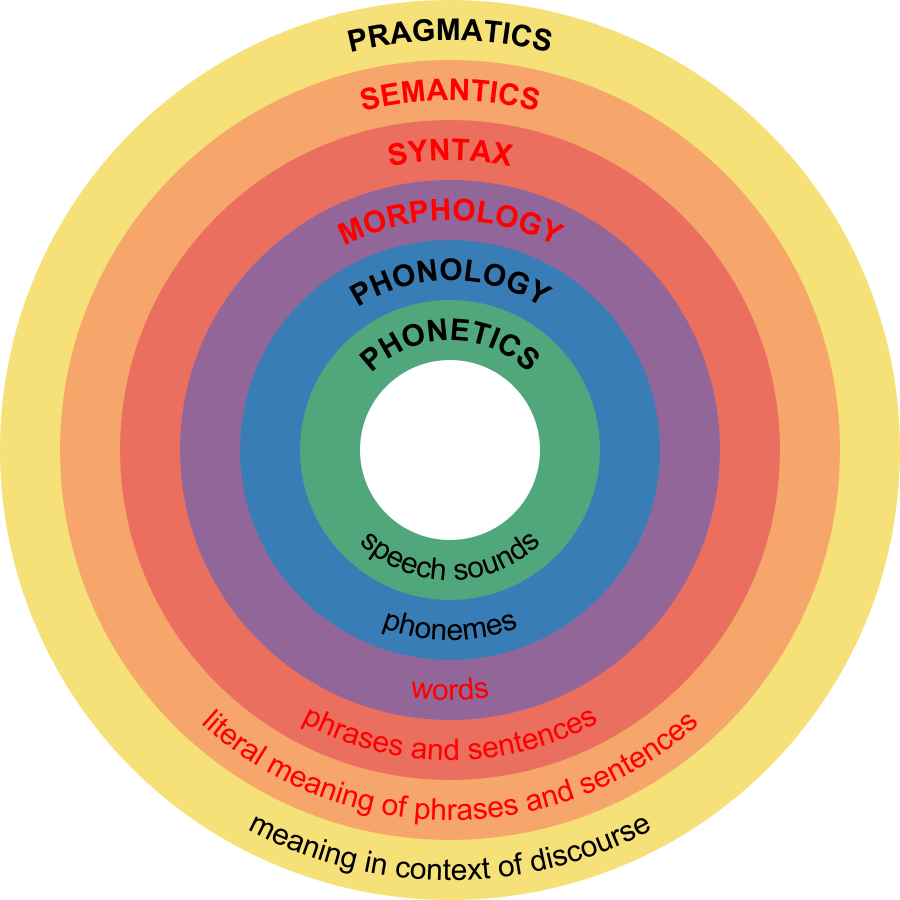
\includegraphics[width=0.5\textwidth]{figures/levels2}
  \end{center}
   
{  \tiny
  Image source: \url{https://commons.wikimedia.org/wiki/File:Major_levels_of_linguistic_structure.svg}
 } 

\end{frame}




\begin{frame}{Linguistic Structures and Graphs}
	
	\begin{itemize}
		\item (Written) language is a \alert{symbolic system}
		\item \textbf{Semantic level}: typed weighted graphs of concepts
		\begin{itemize}
				\item Co-occurrence networks
 
		\item Lexical databases, e.g. WordNet
		\item Thesauri, e.g. NLM
		\item Ontologies, e.g. DBPedia
		\item Associative networks, e.g.  Edinburgh Associative Thesaurus
		\item ...
		
		\end{itemize}
	\end{itemize}	
	
\end{frame}





\begin{frame}{Semantic Graphs}
	
	\begin{center}
  	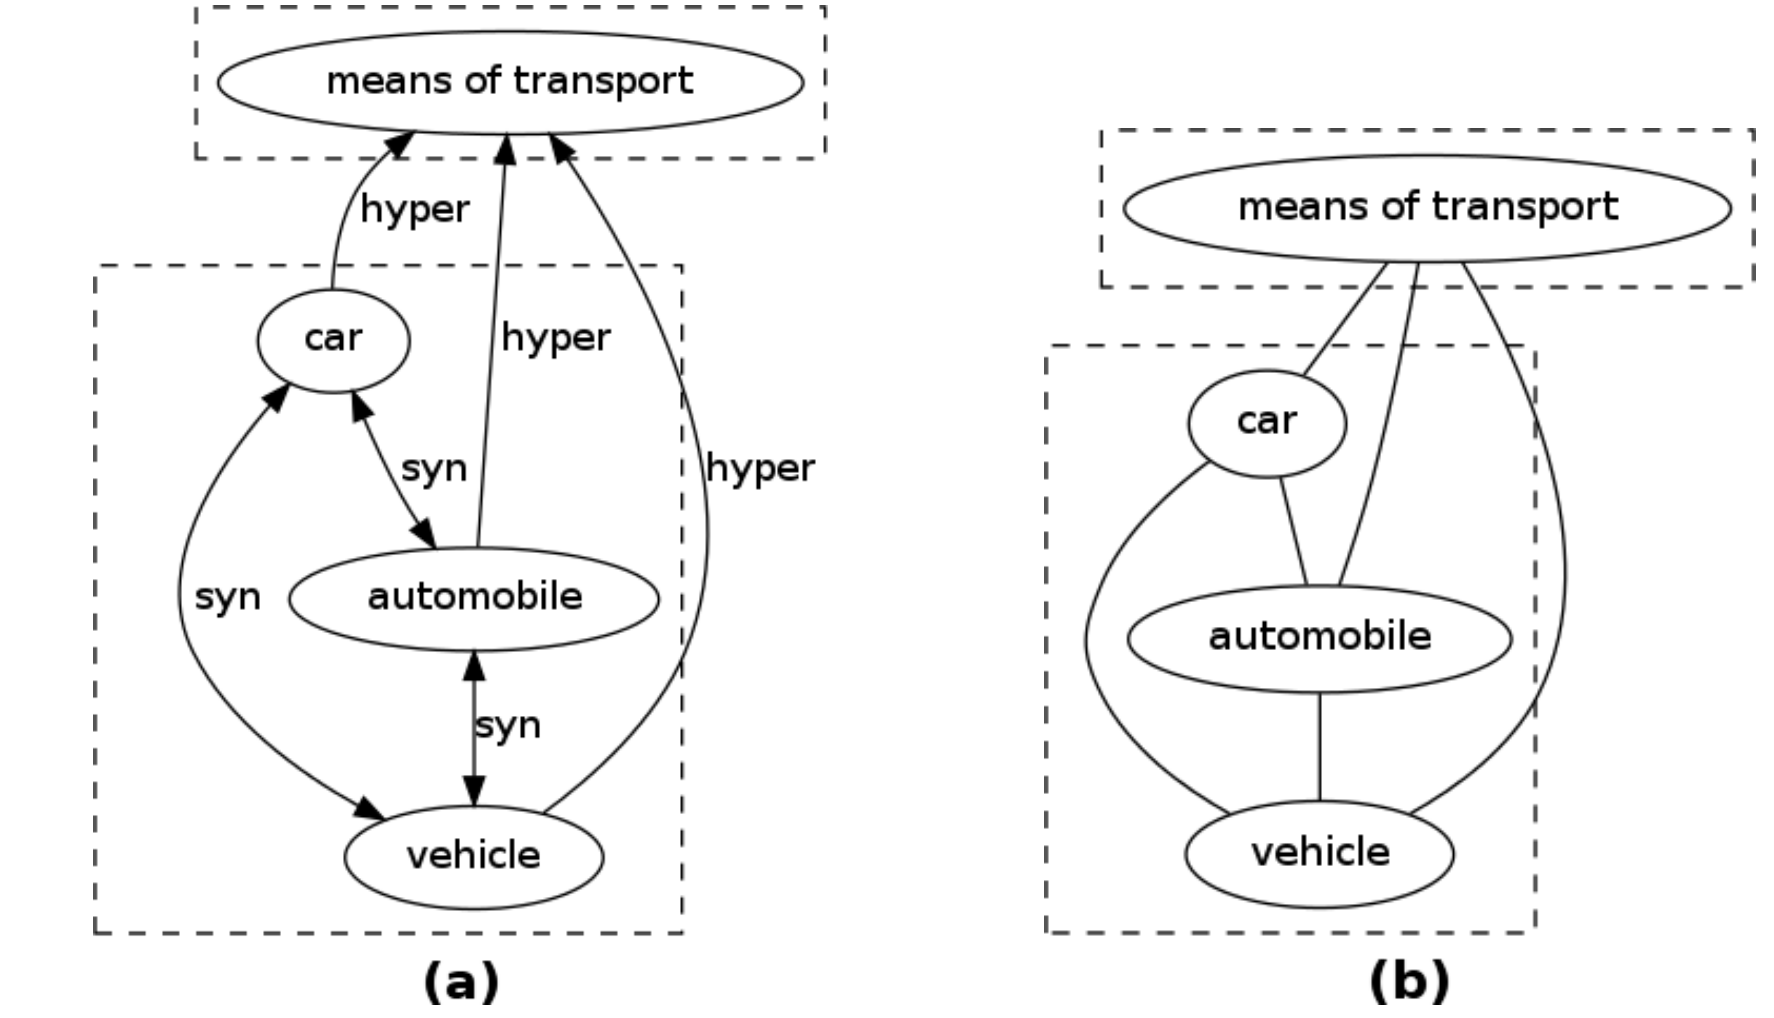
\includegraphics[width=.99\textwidth]{figures/graph1}
  \end{center}	
\end{frame}




\begin{frame}{Semantic Graphs}
	
	\begin{center}
  	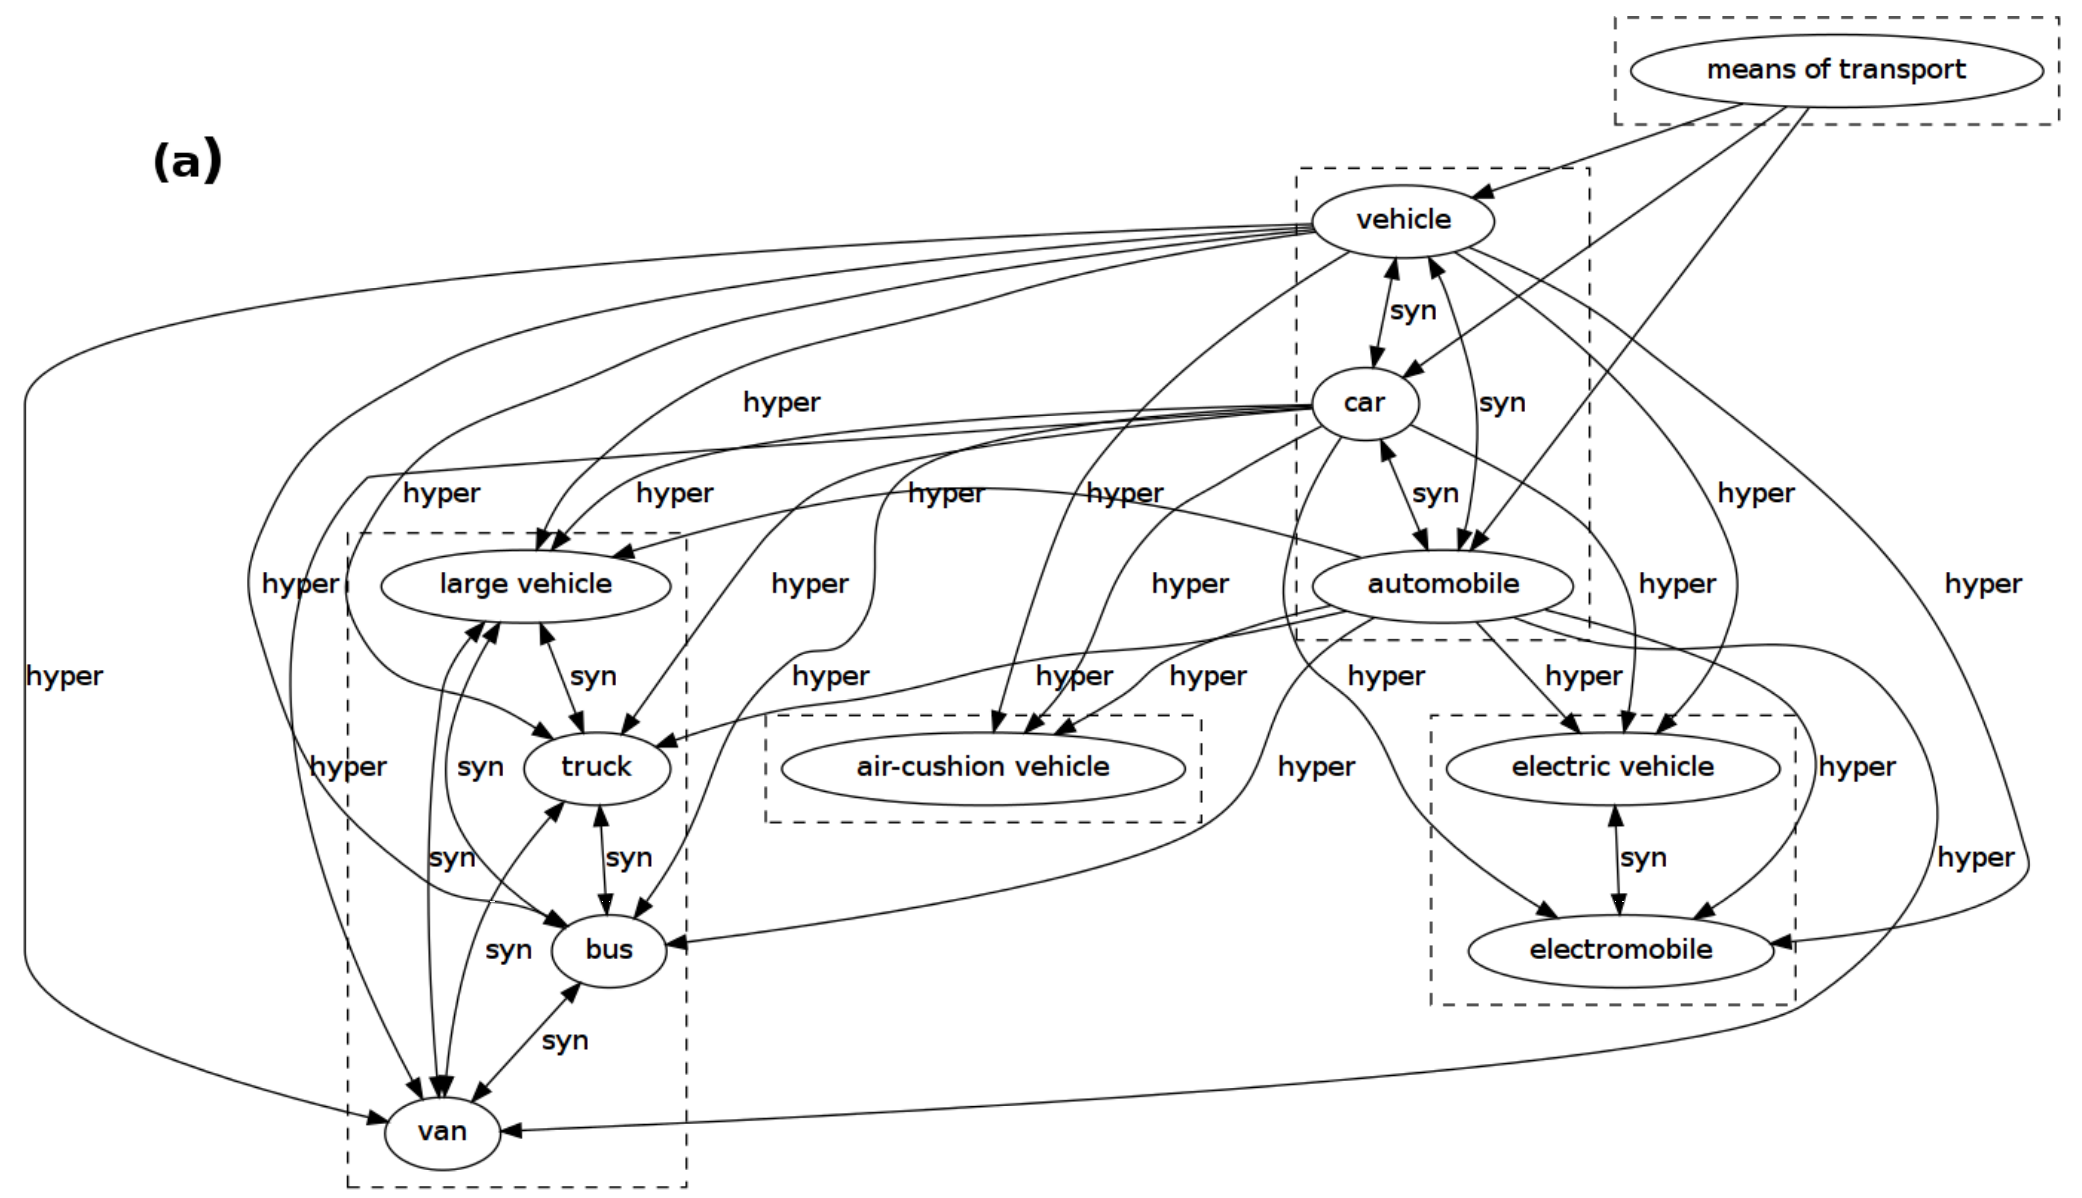
\includegraphics[width=.99\textwidth]{figures/graph2}
  \end{center}	
\end{frame}


\begin{frame}{The new brave world of Deep Learning}
	\vspace{-15pt}
	
	
\begin{columns}
\begin{column}{0.6\textwidth}
   
 \begin{center}
  	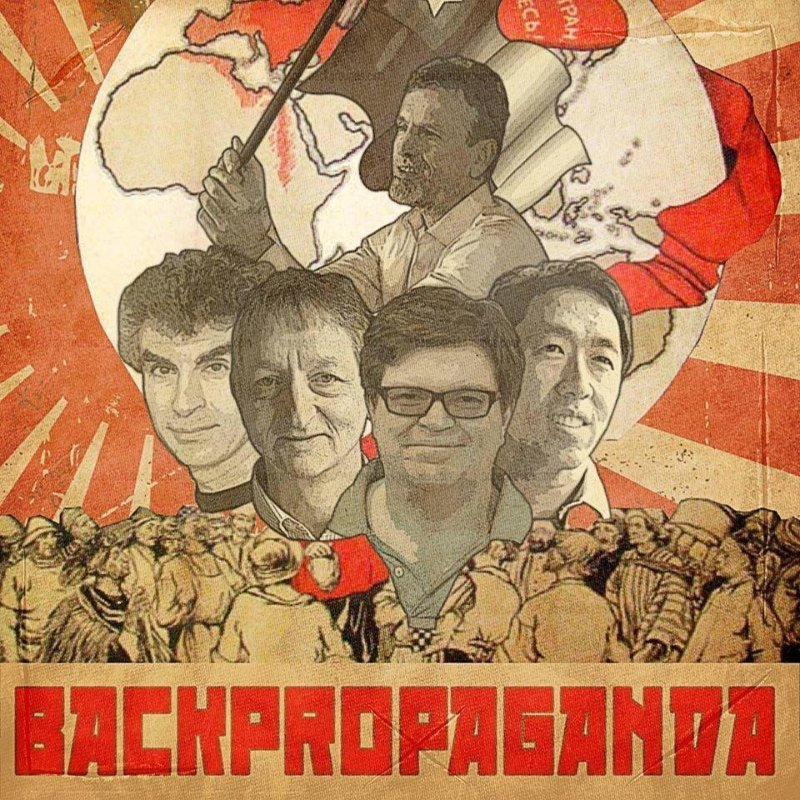
\includegraphics[width=1.0\textwidth]{figures/backprop}
  \end{center}
  
\end{column}
\begin{column}{0.4\textwidth} 
  
 \begin{itemize}
 \item ''Anti-connectivism'' 
 \item End-to-end learning: \alert{symbolic representations aren't needed}
 \pause 
 
 \item Word embeddings lookup (at most)
 	
 \end{itemize}

  
\end{column}
\end{columns}

\end{frame}




\begin{frame}{Graph Matrix Duality}
	\vspace{-25pt}
	
  \begin{center}
  	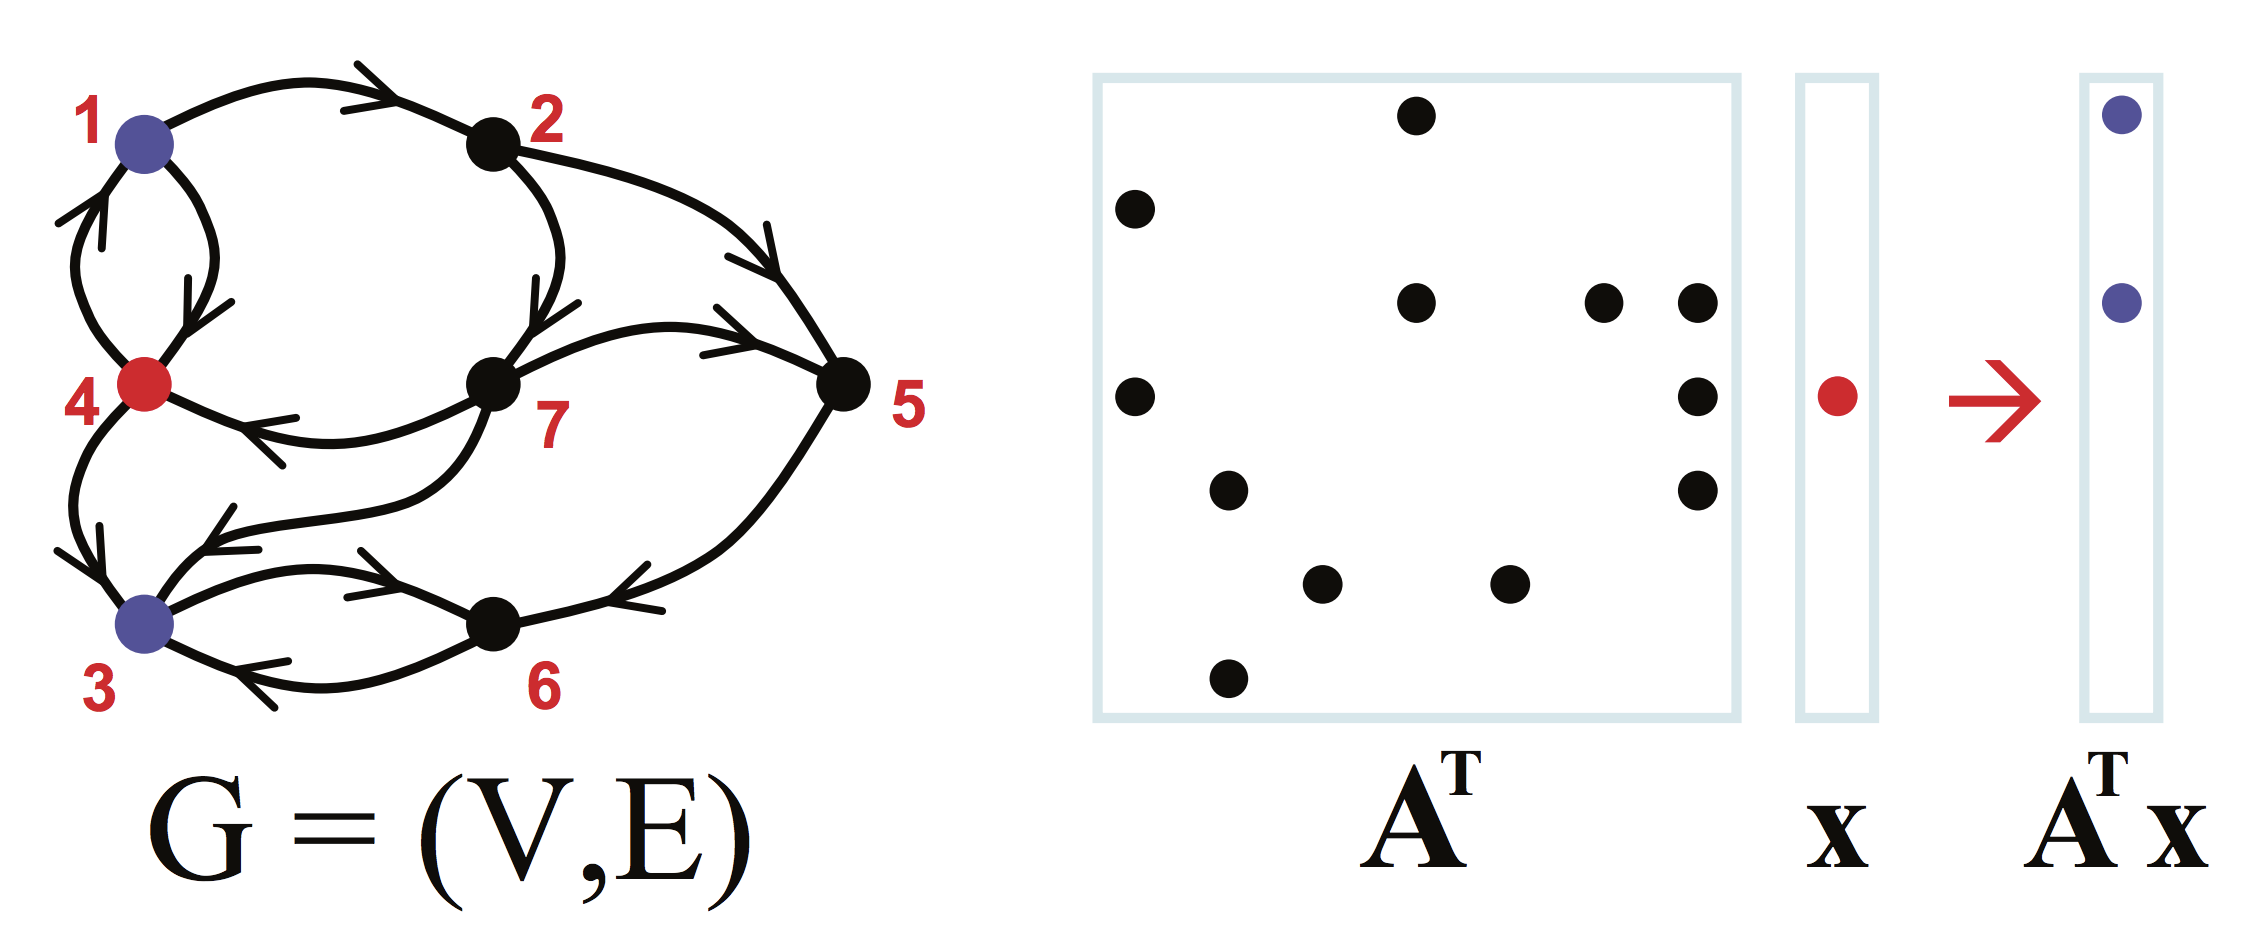
\includegraphics[width=0.99\textwidth]{figures/graph2matrix}
  \end{center}
  
  \pause 

  \begin{itemize}
  	\item   Adjacency matrix $\mathbf{A}$ is dual with the corresponding graph $G$.
  	\pause 
  	\item Vector matrix multiply $\mathbf{A}^T\mathbf{x}$ is dual with breadth-first search.
  \end{itemize}
% 
%{  \footnotesize
%  Image source: \cite{kepner2011graph}
% } 
%
\end{frame}


\begin{frame}{Goal: Linguistic Structures in DL}

  \begin{enumerate}
  	\item \textbf{Learn interpretable symbolic structures from text} in an unsupervised way, which are \alert{more complex than words}.
  	\pause 
  	\item \textbf{Represent the learned structures} in a vector space.
  	\pause 
  	\item \textbf{Use the vector representations} instead/in addition to word embedding the deep learning applications. \alert{Lookup of word senses, frames, etc.}
  	\pause 
  	\item More complex structures could improve performance, but also provide \textbf{better interpretability of the deep learning models}. 
  	
  \end{enumerate}

\end{frame}
